\documentclass[10pt,a4paper]{article}
\usepackage{blindtext}
\usepackage{subcaption}
\usepackage{graphicx}
\usepackage{tikz}
\usepackage{amssymb}
\usepackage{caption}
\usepackage{amsmath}
\usepackage{circuitikz}
\usepackage{hyperref}
\usepackage{amssymb}
\usepackage{amsmath}
\usepackage{listings}

\lstset{
    inputencoding=utf8,
    extendedchars=true,
    literate={á}{{\'a}}1 {é}{{\'e}}1 {í}{{\'i}}1 {ó}{{\'o}}1 {ú}{{\'u}}1 {ñ}{{\~n}}1 {Á}{{\'A}}1 {É}{{\'E}}1 {Í}{{\'I}}1 {Ó}{{\'O}}1 {Ú}{{\'U}}1 {Ñ}{{\~N}}1
}
\usepackage[spanish,activeacute,es-tabla]{babel}
\usepackage[utf8]{inputenc}
\usepackage{ifthen}
\usepackage{listings}
\usepackage{dsfont}
\usepackage{subcaption}
\usepackage{amsmath}
\usepackage[strict]{changepage}
\usepackage[top=1cm,bottom=2cm,left=1cm,right=1cm]{geometry}%
\usepackage{color}%
\newcommand{\tocarEspacios}{%
	\addtolength{\leftskip}{3em}%
	\setlength{\parindent}{0em}%
}

% Especificacion de procs

\newcommand{\In}{\textsf{in }}
\newcommand{\Out}{\textsf{out }}
\newcommand{\Inout}{\textsf{inout }}

\newcommand{\encabezadoDeProc}[4]{%
	% Ponemos la palabrita problema en tt
	%  \noindent%
	{\normalfont\bfseries\ttfamily proc}%
	% Ponemos el nombre del problema
	\ %
	{\normalfont\ttfamily #2}%
	\
	% Ponemos los parametros
	(#3)%
	\ifthenelse{\equal{#4}{}}{}{%
		% Por ultimo, va el tipo del resultado
		\ : #4}
}

\newenvironment{proc}[4][res]{%
	
	% El parametro 1 (opcional) es el nombre del resultado
	% El parametro 2 es el nombre del problema
	% El parametro 3 son los parametros
	% El parametro 4 es el tipo del resultado
	% Preambulo del ambiente problema
	% Tenemos que definir los comandos requiere, asegura, modifica y aux
	\newcommand{\requiere}[2][]{%
		{\normalfont\bfseries\ttfamily requiere}%
		\ifthenelse{\equal{##1}{}}{}{\ {\normalfont\ttfamily ##1} :}\ %
		\{\ensuremath{##2}\}%
		{\normalfont\bfseries\,\par}%
	}
	\newcommand{\asegura}[2][]{%
		{\normalfont\bfseries\ttfamily asegura}%
		\ifthenelse{\equal{##1}{}}{}{\ {\normalfont\ttfamily ##1} :}\
		\{\ensuremath{##2}\}%
		{\normalfont\bfseries\,\par}%
	}
	\renewcommand{\aux}[4]{%
		{\normalfont\bfseries\ttfamily aux\ }%
		{\normalfont\ttfamily ##1}%
		\ifthenelse{\equal{##2}{}}{}{\ (##2)}\ : ##3\, = \ensuremath{##4}%
		{\normalfont\bfseries\,;\par}%
	}
	\renewcommand{\pred}[3]{%
		{\normalfont\bfseries\ttfamily pred }%
		{\normalfont\ttfamily ##1}%
		\ifthenelse{\equal{##2}{}}{}{\ (##2) }%
		\{%
		\begin{adjustwidth}{+5em}{}
			\ensuremath{##3}
		\end{adjustwidth}
		\}%
		{\normalfont\bfseries\,\par}%
	}
	
	\newcommand{\res}{#1}
	\vspace{1ex}
	\noindent
	\encabezadoDeProc{#1}{#2}{#3}{#4}
	% Abrimos la llave
	\par%
	\tocarEspacios
}
{
	% Cerramos la llave
	\vspace{1ex}
}

\newcommand{\aux}[4]{%
	{\normalfont\bfseries\ttfamily\noindent aux\ }%
	{\normalfont\ttfamily #1}%
	\ifthenelse{\equal{#2}{}}{}{\ (#2)}\ : #3\, = \ensuremath{#4}%
	{\normalfont\bfseries\,;\par}%
}

\newcommand{\pred}[3]{%
	{\normalfont\bfseries\ttfamily\noindent pred }%
	{\normalfont\ttfamily #1}%
	\ifthenelse{\equal{#2}{}}{}{\ (#2) }%
	\{%
	\begin{adjustwidth}{+2em}{}
		\ensuremath{#3}
	\end{adjustwidth}
	\}%
	{\normalfont\bfseries\,\par}%
}

% Tipos

\newcommand{\nat}{\ensuremath{\mathds{N}}}
\newcommand{\ent}{\ensuremath{\mathds{Z}}}
\newcommand{\float}{\ensuremath{\mathds{R}}}
\newcommand{\bool}{\ensuremath{\mathsf{Bool}}}
\newcommand{\cha}{\ensuremath{\mathsf{Char}}}
\newcommand{\str}{\ensuremath{\mathsf{String}}}

% Logica

\newcommand{\True}{\ensuremath{\mathrm{true}}}
\newcommand{\False}{\ensuremath{\mathrm{false}}}
\newcommand{\Then}{\ensuremath{\rightarrow}}
\newcommand{\Iff}{\ensuremath{\leftrightarrow}}
\newcommand{\implica}{\ensuremath{\longrightarrow}}
\newcommand{\IfThenElse}[3]{\ensuremath{\mathsf{if}\ #1\ \mathsf{then}\ #2\ \mathsf{else}\ #3\ \mathsf{fi}}}
\newcommand{\yLuego}{\land _L}
\newcommand{\oLuego}{\lor _L}
\newcommand{\implicaLuego}{\implica _L}

\newcommand{\cuantificador}[5]{%
	\ensuremath{(#2 #3: #4)\ (%
		\ifthenelse{\equal{#1}{unalinea}}{
			#5
		}{
			$ % exiting math mode
			\begin{adjustwidth}{+2em}{}
				$#5$%
			\end{adjustwidth}%
			$ % entering math mode
		}
		)}
}

\newcommand{\existe}[4][]{%
	\cuantificador{#1}{\exists}{#2}{#3}{#4}
}
\newcommand{\paraTodo}[4][]{%
	\cuantificador{#1}{\forall}{#2}{#3}{#4}
}

%listas

\newcommand{\TLista}[1]{\ensuremath{seq \langle #1\rangle}}
\newcommand{\lvacia}{\ensuremath{[\ ]}}
\newcommand{\lv}{\ensuremath{[\ ]}}
\newcommand{\longitud}[1]{\ensuremath{|#1|}}
\newcommand{\cons}[1]{\ensuremath{\mathsf{addFirst}}(#1)}
\newcommand{\indice}[1]{\ensuremath{\mathsf{indice}}(#1)}
\newcommand{\conc}[1]{\ensuremath{\mathsf{concat}}(#1)}
\newcommand{\cab}[1]{\ensuremath{\mathsf{head}}(#1)}
\newcommand{\cola}[1]{\ensuremath{\mathsf{tail}}(#1)}
\newcommand{\sub}[1]{\ensuremath{\mathsf{subseq}}(#1)}
\newcommand{\en}[1]{\ensuremath{\mathsf{en}}(#1)}
\newcommand{\cuenta}[2]{\mathsf{cuenta}\ensuremath{(#1, #2)}}
\newcommand{\suma}[1]{\mathsf{suma}(#1)}
\newcommand{\twodots}{\ensuremath{\mathrm{..}}}
\newcommand{\masmas}{\ensuremath{++}}
\newcommand{\matriz}[1]{\TLista{\TLista{#1}}}
\newcommand{\seqchar}{\TLista{\cha}}

\renewcommand{\lstlistingname}{Código}
\lstset{% general command to set parameter(s)
	language=Java,
	morekeywords={endif, endwhile, skip},
	basewidth={0.47em,0.40em},
	columns=fixed, fontadjust, resetmargins, xrightmargin=5pt, xleftmargin=15pt,
	flexiblecolumns=false, tabsize=4, breaklines, breakatwhitespace=false, extendedchars=true,
	numbers=left, numberstyle=\tiny, stepnumber=1, numbersep=9pt,
	frame=l, framesep=3pt,
	captionpos=b,
}

\newcommand{\notimplies}{\;\not\!\!\!\implies}
\title{Algoritmos y Estructuras de Datos III}
\author{Tomás Agustín Hernández}
\date{}

\begin{document}
\maketitle

\begin{figure}[b]
    \centering
    \begin{tikzpicture}[remember picture,overlay]
        \node[anchor=south east, inner sep=0pt, xshift=-1cm, yshift=2cm] at (current page.south east) {
            \begin{minipage}[b]{0.5\textwidth}
                
\includegraphics[width=\linewidth]{logo_uba.jpg}
                \label{fig:bottom}
            \end{minipage}
        };
    \end{tikzpicture}
\end{figure}

\newpage
\section*{Complejidad Computacional (repaso)}
\subsection*{Problema}
Descripción de los datos de entrada y la respuesta a proporcionar para cada uno de los datos de entrada.
\subsection*{Instancia de un Problema}
Es un juego válido de datos de entrada.
\subsection*{Máquina RAM}
Supongamos una Máquina RAM. 
\begin{itemize}
    \item La memoria está dada por una sucesión de celdas numeradas. Cada \textbf{celda} puede almacenar un valor de \textbf{b bits}. 
    \item Supondremos habitualmente que esos \textbf{b bits} de cada celda están fijos, y suponemos que todos los datos que maneja el algoritmo se pueden almacenar con \textbf{b bits}. 
    \textbf{Ej.}: Lo que quiere decir esto es que suponemos que todas las celdas son de 8 bits, y los datos que maneja el algoritmo también son de 8 bits.
    \item Se tiene un programa imperativo que NO está almacenado en memoria que está compuesto por asignaciones y las estructuras de control habituales.
    \item Las asignaciones acceden a las celdas de memoria y realizan las operaciones estándar sobre los tipos de datos primitivos habituales.
\end{itemize}
Cada una de las instrucciones que se ejecuten tienen un tiempo de ejecución asociado
\begin{itemize}
    \item El acceso a cualquier celda de memoria, tanto lectura como escritura es O(1).
    \item Las asignaciones y el manejo de las estructuras de control se realiza en O(1).
    \item Las operaciones entre valores lógicos son O(1).
\end{itemize}
Las operaciones entre enteros/reales dependen de b
\begin{itemize}
    \item Las sumas y restas son O(b).
    \item Las multiplicaciones y divisiones son O(b log b)
\end{itemize}
\textbf{Nota}: Si b está fijo, entonces las operaciones entre enteros/reales es O(1).
\subsection*{Tiempo de Ejecución de un Algoritmo}
Sea A un algoritmo, su tiempo de ejecución es: $T_{A}(I)$ donde esto indica que es la suma de los tiempos de ejecución del algoritmo en una instancia dada I. \\
\textbf{$\longitud{I}$}: Cantidad de bits necesarios para almacenar los datos de entrada de I. \\ \\
\textbf{Nota}: Si \textbf{b está fijo} y la entrada ocupa n celdas de memoria entonces $\longitud{I} = bn = O(n)$
\subsection*{Complejidad de un Algoritmo}
Sea A un algoritmo, su complejidad es: $f_{A}(n) = max_{I:\longitud{I}=n} \ T_{A}(I)$ donde esto indica que la complejidad de un algoritmo A dado un n cualquiera, es el que de mayor tiempo de ejecución tiene en una instancia dada I. 
\subsection*{Cotas}
\textbf{Cota Superior (O)}: $f (n) \in O(g(n)) \iff \exists c \in R>0, n_{0} \in N \ tal \ que \
\forall n \ge n_{0} : f(n) \le c \ast g(n)$  \\
\textbf{Cota Inferior ($\Omega$)}: $f (n) \in \Omega(g(n)) \iff \exists c \in R>0, n_{0} \in N \ tal \ que \ \forall n \ge n_{0} : f(n) \ge c \ast g(n) $ \\
\textbf{Cota Ajustada ($\theta$)}:  $f (n) \in \theta(g(n)) \iff f (n) \in O(g(n)) \ y \ f (n) \in \Omega(g(n)).\ Es \ decir, \ \theta(g(n)) = O(g(n)) \cap \Omega(g(n))$
\subsection*{Tipos de Funciones}
\begin{itemize}
    \item O(n): lineal
    \item $O(n^{2})$: cuadrático
    \item $O(n^{3})$: cúbico
    \item $O(n^{k}) \ k \in \nat$: polinomial. Ej.: $O(n^{4}), \ O(n^{5})$
    \item $O(log \ n)$: logarítmico. 
    \item $O(d^{n}) \ d \in \float_{>1}$: exponencial. Ej.: $ O(2^{n}), \ O(4^{n})$
\end{itemize}
\section*{Algoritmos Satisfactorios y No Satisfactorios}
Un Algoritmo Satisfactorio es un algoritmo que tiene un costo menor a otro. \\
Los algoritmos polinomiales se consideran satisfactorios (cuanto menor sea el grado, mejor). \\
Los algoritmos supra-polinomiales se consideran no satisfactorios. 
\section*{Problema de Optimización}
Sea $x \in S$, un problema de optimización consiste en encontrar la mejor solución dentro de un conjunto: 
\begin{itemize}
    \item $z^{*} = max \ f(x)$
    \item $z^{*} = min \ f(x)$
\end{itemize}
\textbf{Función Objetivo}: Es una función de la forma $f:S\implies \float$
\begin{itemize}
    \item El conjunto S es la \textbf{región factible}.
    \item Los elementos $x \in S$ se llaman \textbf{soluciones factibles}.
    \item El valor $z^{x} \in \float$ es el \textbf{valor óptimo} del problema, y cualquier solución factible $x^{*} \in S \ / \ f(x^{*}) = z^{x}$ se llama un \textbf{óptimo} del problema
\end{itemize}
\section*{Algoritmos de Fuerza Bruta}
También llamado búsqueda exhaustiva o generate and test. 
\begin{itemize}
    \item Genera todas las posibles combinaciones sin importar si se arma una solución correcta o no. Una vez que tiene todas las posibles soluciones, elige de aquellas cuales son las que me sirven para resolver mi problema. 
    \item Lo malo de la fuerza bruta es que de antemano, para saber qué soluciones son correctas debemos encontrar \textbf{todas} inclusive las que no son correctas y esto es súper costoso.
    \item Fácil de implementar.
    \item Algoritmo exacto. Si $\exists$ solución, la encuentra.
    \item Es útil para algoritmos que sabemos que la entrada es pequeña y para verificar correctitud de las soluciones.
    \item Complejidad: Exponencial. 
\end{itemize}

\textbf{Ej.}: Imaginemos que tenemos un tablero de ajedrez y tenemos que buscar las soluciones en las cuales ninguna dama amenace a otra. Una solución por fuerza bruta sería buscar todas las soluciones que existe a cada partida de ajedrez, y de ahí agarrar las que me sirvan. \\ 

\textbf{Ej.}: Imaginemos que tenemos que resolver un Sudoku, si usaramos un casillero de 9x9 y quisieramos aplicar un algoritmo de fuerza bruta, es decir, primero buscar todas las posibles permutaciones 1966270504755529.... posibilidades y de todas estas posibilidades ver cual es solución. Esto es muy tedioso y lento, hay una mejor opción que la fuerza bruta, y es el Backtracking.
\section*{Backtracking}
Es una técnica (de fuerza bruta pero mas eficiente) que consiste en armar un árbol donde debemos extender soluciones parciales \textbf{(cuando noto que una solución parcial (un camino) no me sirve, puedo descartarla e ir a la siguiente sin necesidad de perder más tiempo en esa o sus hijos.)}. \\

Habitualmente se utiliza un vector $ a = (a_{1}, a_{2}, ..., a_{n})$ para representar una \textbf{solución candidata}, donde cada $a_{i} \in A_{i}$ donde $A_{i}$ es un conjunto ordenado y finito. \\ 
En cada paso, se extiende este \textbf{vector a} y se va formando una nueva \textbf{solución parcial} $a = (a_{1}, a_{2}, ..., a_{k})$ con $k<n$  agregando un elemento más que es $a_{k+1} \in S_{k+1} \subseteq A_{k+1}$ al final del vector a. Esto quiere decir que las nuevas soluciones parciales son sucesores directos de la anterior. Si llegamos a un $S_{k+1}$ que es vacío, retrocedemos a la \textbf{solución parcial }$(a_{1}, a_{2}, ..., a_{k-1})$ \\

El espacio de soluciones final consiste en $ A_{1} \ x \ A_{2} \ x \dots \ x \ A_{n} $. \\

Esto último de retroceder podemos verlo como un árbol de decisiones, los cuales si un nodo ya de por sì no me sirve, sus hijos tampoco y vuelvo al nodo anterior para seguir evaluando los demás hijos. \\
\newpage
Entonces...
\begin{itemize}
    \item Conjunto de Soluciones Candidatas: Son todas las combinaciones posibles de los elementos. Pueden ser válidas o no. Son aquellas que habitan el último nivel del árbol (no se pueden extender más) pues no quedan más decisiones por tomar más que considerarlas válidas o inválidas en nuestro problema. Son las hojas del árbol.
    \item Conjunto de Soluciones Parciales: Son todas las combinaciones posibles de los elementos hasta el anteúltimo nivel (si fuese del último sería una solución candidata). Acá se consideran todos los subconjuntos que se van armando en cada paso. Si llegase a haber uno que excede o no cumple lo que necesitamos, no es una solución parcial.
    \item Conjunto de Soluciones Válidas: Son aquellas Soluciones Candidatas que cumplen con lo que buscamos.
\end{itemize}
Preguntar: 
\begin{itemize}
    \item ¿El conjunto de soluciones parciales incluye a quien no es una solucion válida? 
    \item ¿El conjunto de soluciones parciales incluye a las candidatas? En el ej. 1 parece que sí por como lo definen.
\end{itemize}

\[\begin{minipage}[b]{0.7\textwidth}
    \includegraphics[width=\linewidth]{assets/backtracking_arbol1.png}
\end{minipage}\]
Comenzamos evaluando desde la raíz, el nodo de la izquierda cumple hasta ahora nuestra posible solución, nos movemos a ese nodo y luego, evaluando su nodo de la izquierda vemos que se rompe, es decir, alguna restricción que pusimos no se cumple, por lo tanto no tiene sentido seguir explorando las demás soluciones. 
\[\begin{minipage}[b]{0.7\textwidth}
    \includegraphics[width=\linewidth]{assets/backtracking_arbol.png}
\end{minipage}\]
Vemos que efectivamente, habiendo vuelto a la raíz, ahora sí encontramos un camino mejor que el camino del nodo de la izquierda. Por lo tanto, podemos seguir evaluando hacia abajo. \\
Véase \hyperref[subsec:backtracking_ex]{\underline{anexo}} para un ejemplo didáctico.
\subsection*{Podas}
Nos permiten descartar configuraciones.\\
\textbf{Podas por factibilidad}: Evito explorar nodos no factibles. Esto quiere decir que:
\begin{itemize}
    \item Si veo que al evaluar el próximo nodo del camino ya no es solución retrocedo inmediatamente al paso anterior.
    \item Esto de volver al paso anterior, básicamente lo que estoy haciendo es matar al nodo que no me sirve y a los hijos de ese nodo. Si tengo $\{ a_{1} \rightarrow a_{2} \rightarrow a_{3}\}$ pero a la hora de evaluar veo que $a_{1}$ no me sirve, por dominó tampoco me sirven $a_{2}$ ni $a_{3}$
\end{itemize}
\textbf{Podas por optimalidad}: Evito explorar nodos subóptimos. Esto quiere decir que: 
\begin{itemize}
    \item Si veo que al evaluar el próximo nodo del camino, ya no forma la mejor solución entonces retrocedo inmediatamente al paso anterior.
    \item \textbf{Importante}: En las podas por optimalidad se necesita un criterio más para saber qué seria considerada una mejor solución que otra. Un ejemplo puede ser un problema de un viajante de comercio que debe encontrar el camino de menor costo para visitar todas las ciudades. A medida que encuentro una solución entera, puedo ir buscando otras y comparándolas. Si en algún momento veo que ya se pasó (tiene un costo mayor que la solución anterior encontrada) de la solución entera la descarto. Es algo más estimativo.
\end{itemize}

El éxito del backtracking depende de las podas. \\
\textbf{Branch and bound} 
\begin{itemize}
    \item Separo en subproblemas con un límite inferior/superior del valor óptimo que puede obtenerse en ese subproblema.
    \item La poda se realiza al comparar los límites inferior/superior de los subproblemas con el mejor valor óptimo conocido. Si el límite inferior/superior de un subproblema es peor que la mejor solución conocida, ese subproblema es podado.
    \item El objetivo de branch and bound es encontrar la solución más óptima al problema.
\end{itemize}
Backtracking garantiza encontrar al menos una solución válida y luego optimiza, mientras que branch and bound está diseñado para encontrar la mejor solución posible de manera más eficiente desde el principio utilizando límites para podar ramas del espacio de búsqueda.
\subsection*{Soluciones}
\textbf{Todas las soluciones}:
\begin{lstlisting}
    algoritmo BT(a,k)
        si a es solución entonces
            procesar(a)
            retornar
        sino
            para cada a' en Sucesores(a,k)
            BT(a', k + 1)
            fin para
        fin si
        retornar
\end{lstlisting}
\textbf{Una solución}:
\begin{lstlisting}
    algoritmo BT(a,k)
    si a es solución entonces
        sol <- a
        encontro <- true
    sino
        para cada a' en Sucesores(a,k)
            BT(a', k + 1)
            si encontro entonces
                retornar
            fin si
        fin para
    fin si
    retornar
\end{lstlisting}
\textbf{Ej.}: Resolver un sudoku se resuelve en forma muy eficiente con un algoritmo de backtracking.
\subsection*{Casos de Uso de Backtracking}
\begin{itemize}
    \item Problemas de Decisión.
    \item Problemas de Optimización: Encontrar la mejor solución.
    \item Problemas de Enumeración: Todas las soluciones factibles a un problema.
\end{itemize}
\section*{Programación Dinámica}
Consiste en reutilizar valores previamente calculados para ahorrar tiempo. \textbf{¿Cuál es el costo?}, el costo es que acá \textbf{usamos más espacio de la memoria}. \\

\textbf{Nota}: Si queremos sacar ventaja de la memorización \textbf{tenemos que acceder al valor guardado en la estructura de datos en O(1) o en un menor tiempo que lo que costaría calcularlo} otra vez. \\

Aunque no lo parezca, guardar información que vamos a terminar reutilizando ahorra mucho tiempo. \\

Normalmente, la programación dinámica se utiliza cuando de antemano ya sabemos que vamos a tener que terminar reutilizando valores que ya previamente calculamos para esos parámetros de entrada. A esto se le llama \textbf{superposición de estados} y ocurre cuando un árbol de llamadas recursivas resuelve el mismo problema para mismos parámetros de entrada. \\

Veamos ahora dos formas de encarar un problema de programación dinámica 

\subsection*{Enfoque Top-Down} 
Se implementa recursivamente. La idea es ir guardando el resultado de cada llamada recursiva en una estructura de datos \textbf{(memorización)}. Si llegase a suceder que en una nueva llamada vemos que esa llamada ya ocurrió previamente con los mismos parámetros podemos devolver el valor previamente calculado almacenado en la estructura de datos.  \\ 

Una forma de visualizarlo es con el árbol de llamados. Si tenemos una función $f(n, k)$ definida como $f(n, k) = f(n-1, k) + f(n, k-1)$ con $k<n$ podríamos representar el pensamiento top-down de la siguiente manera
\[\begin{minipage}[b]{0.7\textwidth}
    \includegraphics[width=\linewidth]{assets/top_down.png}
\end{minipage}\]
Claramente podemos observar como $f(n-1, k-1)$ se repite de ambos lados del árbol. Si esto fuese costoso de calcular, estaríamos perdiendo tiempo en algo que podríamos haber guardado. \\

El nombre de Top-Down viene del lado que partimos del problema más grande y terminamos llegando a un caso base.
Véase \hyperref[subsec:top_down_programacion_dinamica]{\underline{anexo}} para ver qué tanto mejora el tiempo de ejecución
\subsection*{Enfoque Bottom-Up}
Generalmente es iterativo, pero no siempre. Empieza resolviendo las partes más pequeñas y fundamentales del problema. Cada vez que resuelve un problema, almacena su solución en una estructura de datos auxiliar.
\section*{Divide \& Conquer}
Esta técnica consiste en dividir \textbf{un problema en subproblemas
 del mismo tipo} que en el original, resolver los subproblemas y luego combinar las soluciones. \\

\textbf{Importante}: Cuando hablamos de subproblemas, hablamos de subproblemas necesariamente más chicos que el problema original; Deben ser todos del mismo tipo y no podemos resolver diferentes subproblemas. \\

Ej.: Si tengo una pared enorme, la puedo pintar por partes. Si a la primera la pinté de arriba hacia abajo la segunda la voy a pintar igual y exactamente con los mismos movimientos. Al final de todo, veré que la pared quedó perfectamente pintada.
El ejemplo representa claramente un problema de Divide \& Conquer pues
\begin{itemize}
    \item Al ser un problema grande, divido la tarea de pintar la pared enorme en partes iguales de una manera más sencilla y llevadera.
    \item Las paredes las pinto a todas de arriba hacia abajo y con exactamente los mismos movimientos (subproblemas del mismo tipo).
    \item Como sé que la porción de pared anterior quedó perfectamente pintada y la siguiente también lo estará, entonces terminaré pintando la pared entera.
\end{itemize}

\textbf{Importante}: Divide \& Conquer debería tener una complejidad parecida a resolver el problema original. Si resolver el problema original nos cuesta $O(n)$ y con esta técnica $O(n^{3})$ algo anda mal porque el tiempo de resolución debería ser igual (o menor) separando y resolviendo los subproblemas.
\subsection*{Teorema Maestro}
Nos permite calcular la complejidad temporal de un un algoritmo que involucra recursión.
\[T(n) = \left\{ \begin{array}{lcc} a \ast T(n/c) + f(n) & si & n>1  \\ 1 & si & n=1 \end{array} \right.\]
Donde: 
\begin{itemize}
    \item a: cantidad de subproblemas en los que el problema se divide.
    \item n/c: es el tamaño de cada subproblema.
    \item c: cantidad de problemas.
    \item T(n/c): Es el tiempo de ejecución del algoritmo para un problema de tamaño n/c.
    \item f(n): Costo de dividir el problema y combinar los resultados de los subproblemas.
\end{itemize}
\subsection*{Casos del Teorema Maestro}
\begin{itemize}
    \item Si $f(n) = O(n^{log_{c} a-\epsilon})$ con $\epsilon >$ 0, entonces $T(n) = \Theta(n^{log_{c} \ a})$
    \item Si $f(n) = \Theta(n^{log_{c} a})$ entonces $T(n) = \Theta(n^{log_{c} a} \ log \ n)$
    \item Si $f(n) = \Omega(n^{log_{c} \ a + \epsilon})$ para $\epsilon$ $>$ 0, y si $ af(\frac{n}{c}) < kf(n)$ para $k<1$ y para n suficientemente grandes, entonces $T(n) = \Theta(f(n))$
\end{itemize}
\subsection*{Qué no puede pasar en el Teorema Maestro}
\begin{itemize}
    \item f(n) no puede ser negativo porque es el tiempo que tarda el algoritmo. Siempre es positivo.
    \item a es una constante positiva pues el número de subproblemas una vez que arranca la recursión es fija.
\end{itemize}
\section*{Heurísticas}
Es un procedimiento computacional que intenta obtener soluciones de buena calidad para un problema y que su comportamiento sea preciso. \\
Decimos que A es un algoritmo $\epsilon$-aproximado $(\epsilon \ge 0)$ para un problema si \[\longitud{\frac{X_{A} - X_{OPT}}{X_{OPT}}} \le \epsilon\]
\section*{Algoritmos Golosos (Algoritmos Greedy)}
Es una técnica que consiste en elegir en cada paso la mejor opción sin considerar lo que pueda pasar después. \\
Saber cual es la mejor opción depende de qué nos pidan como prioritario. \\
\textbf{¿A qué me refiero como prioritario?}
\begin{itemize}
    \item Si te pido que de una lista de 100 películas, tomes la mayor cantidad de películas para que yo vea en 8hs: La idea sería que tomes las películas con menor duración (porque a menor duración, mas películas vas a elegir)
    \item Si te pido que vayas a la panadería y traigas 4kg de pan: No se puede resolver con greedy, porque no te especifico cuál sería el pan ideal.
\end{itemize}
Veamos algunos ejemplos más
\begin{itemize}
    \item Tengo monedas de 1, 5, 10 y 25 centavos. Debo dar $0.69$ de vuelto con la \textbf{menor cantidad de monedas}. 
    \begin{itemize}
        \item IDEA: La mejor elección en este caso que tengo que devolver menor cantidad de monedas, me conviene devolver más monedas de la moneda con mayor valor. 
        \item Toma 1 moneda de 25 pues sumando lo que tengo sucede que $0.25<0.69$.
        \item Toma 1 moneda de 25 pues sumando lo que tengo sucede que $0.50<0.69$
        \item Toma 1 moneda de 25 $0.75<0.69$ es falso, por lo que sigo teniendo $0.50$.
        \item Toma 1 moneda de 10 pues sumando lo que tengo sucede que $0.60<0.69$.
        \item Toma 1 moneda de 10 $0.70<0.69$ es falso, por lo que sigo teniendo $0.60$.
        \item Toma 1 moneda de 5 pues sumando lo que tengo sucede que $0.65<0.69$.
        \item Toma 1 moneda de 5 $0.70<0.69$ es falso, por lo que sigo teniendo $0.65$.
        \item Toma 1 moneda de 1 (4 veces) pues sumando lo que tengo sucede que $0.69<0.69$
    \end{itemize}
    \item Un servidor tiene n clientes para atender, los puede atender en cualquier orden. El objetivo es determinar en que orden se deben atender los clientes para \textbf{minimizar la suma de los tiempos de espera} de los clientes. 
    \begin{itemize}
        \item Me pongo en situación: Supongamos que tenemos 1000 clientes. Tenemos 2 representantes, 2 de los clientes tienen problemas que se resuelven en 4hs. Los demás, tienen problemas pero se resuelven en poco tiempo. IDEA: Ordeno los clientes por tiempo de demora de sus trámites y voy resolviendo los más cortos. Esto producirá que los clientes se vayan contentos porque se los atiende rápido (pues sabemos que a la larga, la suma de los tiempos de los trámites de los clientes con trámites cortos, es igual o menor a atender a solo los 2 clientes).
        \item Mal camino: Si priorizaramos a los clientes que tienen trámites más largos tendríamos 998 clientes enojados. 
        \item Buen camino: Si priorizaramos a los 998 clientes aunque los otros dos hayan llegado antes, seguramente ellos estén enojados pero es mejor tener 998 felices que solo 2.
    \end{itemize}
\end{itemize}

Esto demuestra que los Algoritmos Golosos nos dan solución para \textbf{minimizar el tiempo total de espera en un sistema atendiendo por menor tiempo de atención} y también \textbf{minimizar la cantidad de monedas que devolvemos, pero seguramente tendremos más monedas de mayor valor}.
\section*{Grafos}
\section*{Anexo}
\subsection*{Backtracking}
\label{subsec:backtracking_ex}
\[\begin{minipage}[b]{1\textwidth}
    \includegraphics[width=\linewidth]{assets/ex_backtracking_1.png}
\end{minipage}\]
El ejercicio nos plantea la idea de que necesitamos de alguna manera saber qué combinaciones de subconjuntos son válidas tal que la suma de sus elementos internos da k = 12. \\
Por lo que se nos indica, cada una de estas combinaciones está formada de manera binaria, es decir, siendo $ C = \{6, 12, 6\}$ si yo tengo el subconjunto $\{1, 0, 0\}$ eso indicaría que la suma que da los elementos del subconjunto es 6. \\
Lo primero que tenemos que hacer es plantear el árbol entero ¿por qué? porque necesitamos de alguna manera ver \textbf{todas} las soluciones candidatas que tenemos. \\
\[\begin{minipage}[b]{1\textwidth}
    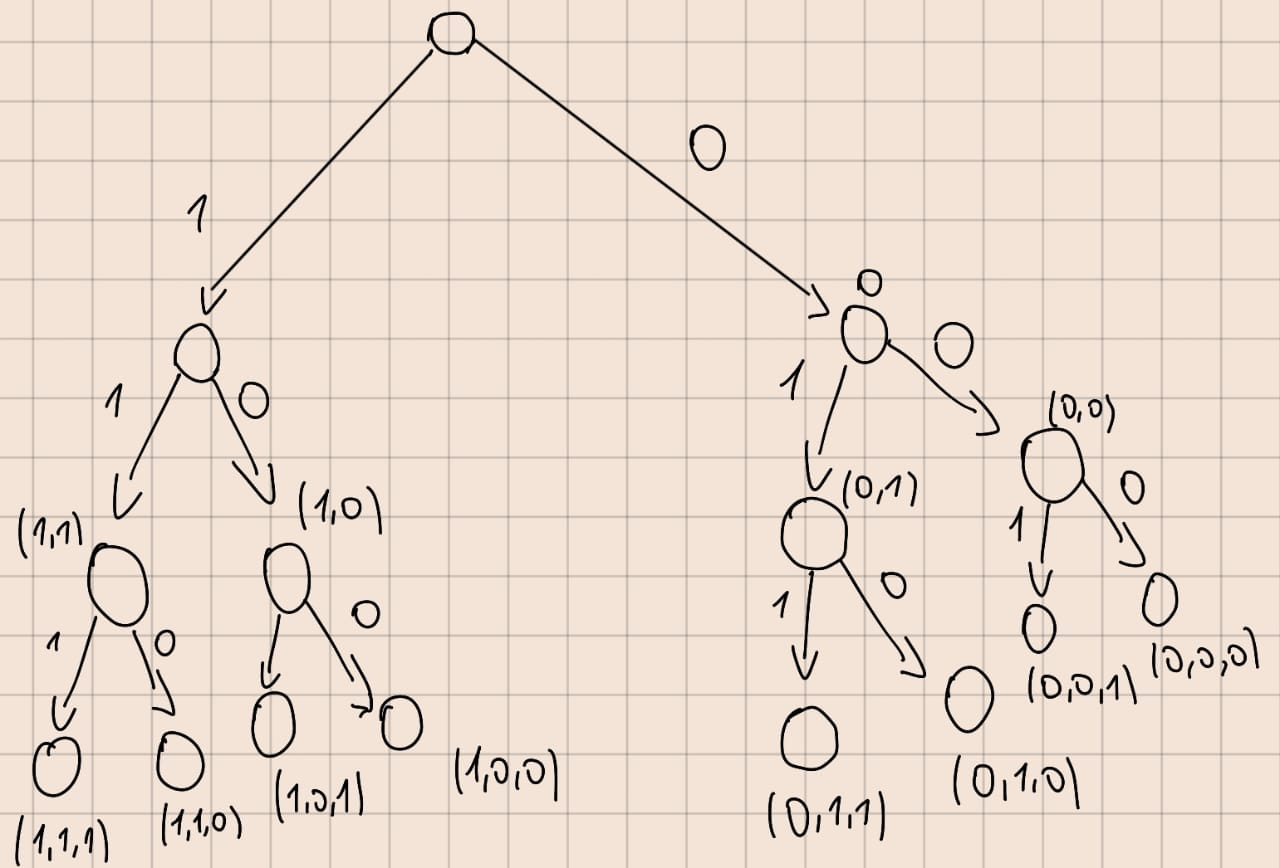
\includegraphics[width=\linewidth]{assets/ex_backtracking_dibujo_arbol.jpg}
\end{minipage}\]
Así, las \textbf{Soluciones Candidatas} son las del último nivel: \\
Por lo tanto $\{(1, 1, 1), (1, 1, 0), (1,0,1), (1,0,0), (0,1,1), (0,1,0), (0,0,1), (0,0,0)\}$ \\
Luego, las \textbf{Soluciones Parciales} son aquellas que hasta el anteúltimo nivel son válidas: \\
Por lo tanto $\{(0), (1), (1,0), (0,1), (0, 0), (1, 1)\}$ \\
Por último, las \textbf{Soluciones Válidas} son aquellas que cumplen con nuestra condición en las Soluciones Candidatas. \\
Por lo tanto $\{(0,1,0), (1,0,1)\}$ \\

En este ejercicio hacemos podas por factibilidad pues, si la suma de los elementos excede 12 todo el camino que sigue es inválido.



\subsection*{Programación Dinámica en C++ (Top-Down)}
\label{subsec:top_down_programacion_dinamica}
\textbf{Importante}: Notar que estoy usando long long porque los números que puede tomar fibonacci son tan grandes, que evito correr riesgos con int. \\
\textbf{Importante}: Notar que estoy envíando el vector por referencia. De lo contrario, se generaría uno nuevo en cada llamada. \\
\begin{lstlisting}
Con memorización
    #include <iostream>
    #include <vector>
    #include <chrono>
    using namespace std::chrono;

    long long fibonacci(long long n, std::vector<long long>& memo)
    {
        if (memo[n] != -1)
        {
            return memo[n];
        }

        if (n == 0)
        {
            return 0;
        }
        else if (n == 1)
        {
            return 1;
        }

        memo[n] = fibonacci(n - 1, memo) + fibonacci(n - 2, memo);
        return memo[n];
    }

    int main()
    {
        auto start = high_resolution_clock::now();
        int n = 0;
        std::cout << "Ingrese un numero para calcular fibonacci" << std::endl;
        std::cin >> n;
        std::vector<long long> memo(n + 1, -1);
        long long fibo = fibonacci(n, memo);
        std::cout << "Fibonacci de " << n << " es " << fibo << std::endl;

        // chrono
        auto stop = high_resolution_clock::now();
        auto duration = duration_cast<microseconds>(stop - start);
        std::cout << "El tiempo de ejecucion es: " << duration.count() << " milisegundos" << std::endl;

        return 0;
    }
    
Fibo 50 (12586269025): 2887439 milisegundos.
\end{lstlisting}
\begin{lstlisting}
Sin memorización
    #include <iostream>
    #include <vector>
    #include <chrono>
    using namespace std::chrono;

    long long fibonacci(int n)
    {
        
        if (n == 0)
        {
            return 0;
        }
        else if (n == 1)
        {
            return 1;
        }
        
        return fibonacci(n - 1) + fibonacci(n - 2);
    }

    int main()
    {
        auto start = high_resolution_clock::now();
        int n = 0;
        std::cout << "Ingrese un numero para calcular fibonacci" << std::endl;
        std::cin >> n;
        long long fibo = fibonacci(n);
        std::cout << "Fibonacci de " << n << " es " << fibo << std::endl;

        // chrono
        auto stop = high_resolution_clock::now();
        auto duration = duration_cast<microseconds>(stop - start);
        std::cout << "El tiempo de ejecucion es: " << duration.count() << " milisegundos" << std::endl;

        return 0;
    }
Fibo 50: ? milisegundos. No termina, se cuelga.
\end{lstlisting}
\end{document} 
